\renewcommand*{\arraystretch}{1.1}

\subsection*{Interactive / complex / 8}
\label{section:interactive-complex-read-08}

% change \emph{} to use sans-serif font
\let\oldemph\emph
\renewcommand{\emph}[1]{{\footnotesize \sf #1}}

\renewcommand{\currentQueryCard}{8}
\marginpar{
	\raggedleft
	\vspace{0.22ex}

    \queryRefCard{interactive-complex-read-01}{Interactive}{1}\\
    \queryRefCard{interactive-complex-read-02}{Interactive}{2}\\
    \queryRefCard{interactive-complex-read-03}{Interactive}{3}\\
    \queryRefCard{interactive-complex-read-04}{Interactive}{4}\\
    \queryRefCard{interactive-complex-read-05}{Interactive}{5}\\
    \queryRefCard{interactive-complex-read-06}{Interactive}{6}\\
    \queryRefCard{interactive-complex-read-07}{Interactive}{7}\\
    \queryRefCard{interactive-complex-read-08}{Interactive}{8}\\
    \queryRefCard{interactive-complex-read-09}{Interactive}{9}\\
    \queryRefCard{interactive-complex-read-10}{Interactive}{10}\\
    \queryRefCard{interactive-complex-read-11}{Interactive}{11}\\
    \queryRefCard{interactive-complex-read-12}{Interactive}{12}\\
    \queryRefCard{interactive-complex-read-13}{Interactive}{13}\\
    \queryRefCard{interactive-complex-read-14}{Interactive}{14}\\
}

\noindent\begin{tabularx}{\queryCardWidth}{|>{\queryPropertyCell}p{\queryPropertyCellWidth}|X|}
	\hline
	query & Interactive / complex / 8 \\ \hline
%
	title & Recent replies
 \\ \hline
%
	pattern & \hfill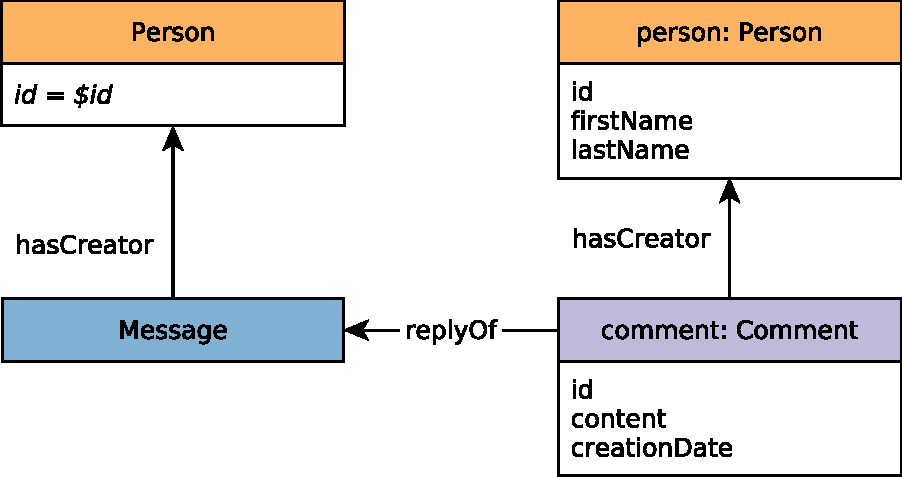
\includegraphics[scale=\patternscale,margin=0cm .2cm]{patterns/interactive-complex-read-08}\hfill\vadjust{} \\ \hline
%
	desc. & Given a start Person, find (most recent) Comments that are replies to
Messages of the start Person. Only consider immediate (1-hop) replies,
not the transitive (multi-hop) case. Return the reply Comments, and the
Person that created each reply Comment.
 \\ \hline
%
	
		params &
		\innerCardVSpace{\begin{tabularx}{\attributeCardWidth}{|>{\paramNumberCell}c|>{\varNameCell}M|>{\typeCell}m{\typeWidth}|Y|} \hline
		$\mathsf{1}$ & Person.id
 & ID
 &  \\ \hline
		\end{tabularx}}\innerCardVSpace \\ \hline
	
%
	
		result &
		\innerCardVSpace{\begin{tabularx}{\attributeCardWidth}{|>{\resultNumberCell}c|>{\varNameCell}M|>{\typeCell}m{\typeWidth}|>{\resultOriginCell}c|Y|} \hline
		$\mathsf{1}$ & Person.id & ID & R &
				 \\ \hline
		$\mathsf{2}$ & Person.firstName & String & R &
				 \\ \hline
		$\mathsf{3}$ & Person.lastName & String & R &
				 \\ \hline
		$\mathsf{4}$ & Comment.creationDate & DateTime & R &
				 \\ \hline
		$\mathsf{5}$ & Comment.id & ID & R &
				 \\ \hline
		$\mathsf{6}$ & Comment.content & String & R &
				 \\ \hline
		\end{tabularx}}\innerCardVSpace \\ \hline
	
%
	
		sort		&
		\innerCardVSpace{\begin{tabularx}{\attributeCardWidth}{|>{\sortNumberCell}c|>{\varNameCell}M|>{\directionCell}c|Y|} \hline
		$\mathsf{1}$ & Comment.creationDate
 & $\desc
$ &  \\ \hline
		$\mathsf{2}$ & Comment.id
 & $\asc
$ &  \\ \hline
		\end{tabularx}}\innerCardVSpace \\ \hline
	%
	limit & 20 \\ \hline
	%
	CPs &
	\multicolumn{1}{>{\raggedright}l|}{
		\chokePoint{2.4}, 
		\chokePoint{3.2}, 
		\chokePoint{3.3}, 
		\chokePoint{5.3}
		} \\ \hline
	%
	relevance &
		\small This query looks for paths of length two, starting from a given Person, going through its created Messages and
finishing at their replies. In this query there is temporal locality between the replies being accessed. Thus the top k
order by this can interact with the selection, i.e. do not consider older posts than the 20th oldest seen so far.
 \\ \hline%
\end{tabularx}
\queryCardVSpace

% change \emph back to the old one
\renewcommand{\emph}[1]{\oldemph{#1}}